%%%%%%%%%%%%%%%%%%%%%%%%%%%%%%%%%%%%%%%%%%%%%%%%%%%%%%%%%%%%%%%%%%%%%%%%
% Plantilla TFG/TFM
% Escuela Politécnica Superior de la Universidad de Alicante
% Realizado por: Jose Manuel Requena Plens
% Contacto: info@jmrplens.com / Telegram:@jmrplens
%%%%%%%%%%%%%%%%%%%%%%%%%%%%%%%%%%%%%%%%%%%%%%%%%%%%%%%%%%%%%%%%%%%%%%%%

\chapter{Development}\label{development}
\section{Data}

We developed a data cleaning pipeline using the pandas library. This pipeline
fixes some errors in the data, removes outliers and sessions with missing
measurements.

\section{Body representation}

We extracted \gls{smpl} parameters --- shape ($\beta$) and pose ($\theta$) ---
from the 3D scans using a custom minimization algorithm.

\section{Neural network architecture}

We used the PyTorch library to implement our custom neural network
architecture.

\begin{figure}
    \centering
    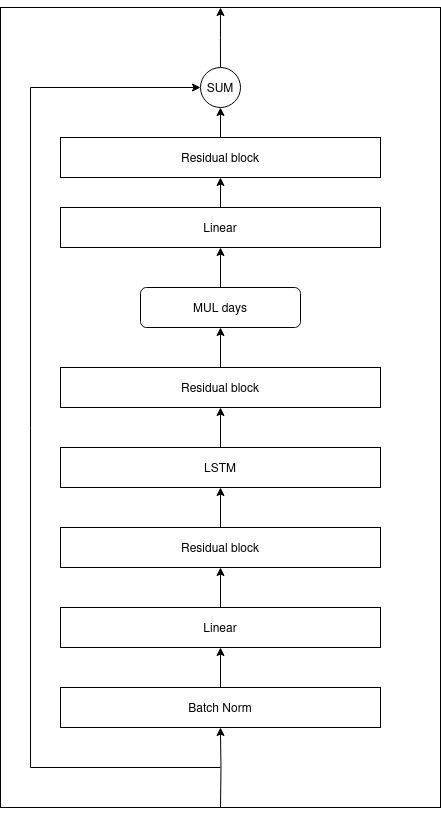
\includegraphics[width=6cm]{files/nn_diagram}
    \caption{Diagram of the neural network architecture}
\end{figure}

This architecture can handle temporal data of varying lengths.

\section{Training}

The neural network inputs a tensor of shape (batch size, max sequence length,
number of features), a tensor of shape (batch size, 1) containing the length of
the current sequence, and a scalar representing the number of days until the
next session. It returns a tensor of shape (batch size, max sequence length,
number of features) containing the predicted values for the next session.

\begin{itemize}
    \item The neural network takes as input:
          \begin{itemize}
              \item A tensor of shape (batch size, max sequence length, number of features).
              \item A tensor of shape (batch size, 1) containing the length of the current
                    sequence.
              \item A scalar representing the number of days until the next session.
          \end{itemize}
    \item The neural network returns:
          \begin{itemize}
              \item A tensor of shape (batch size, max sequence length, number of features) that
                    contains the predicted values for the next session.
          \end{itemize}
\end{itemize}

For features, we concatenate the \gls{smpl} parameters shape ($\beta$) with the
patient's height, weight, and age. We also experimented with using body fat
percentage and muscle mass percentage, but the results were comparable. We used
the AdamW optimizer with a variable learning rate and weight decay, and MSE
loss.

\section{Evaluation}

The mean absolute error (MAE) of the predicted betas served as our evaluation
metric.

\section{Results}

\begin{figure}[h]
    \centering
    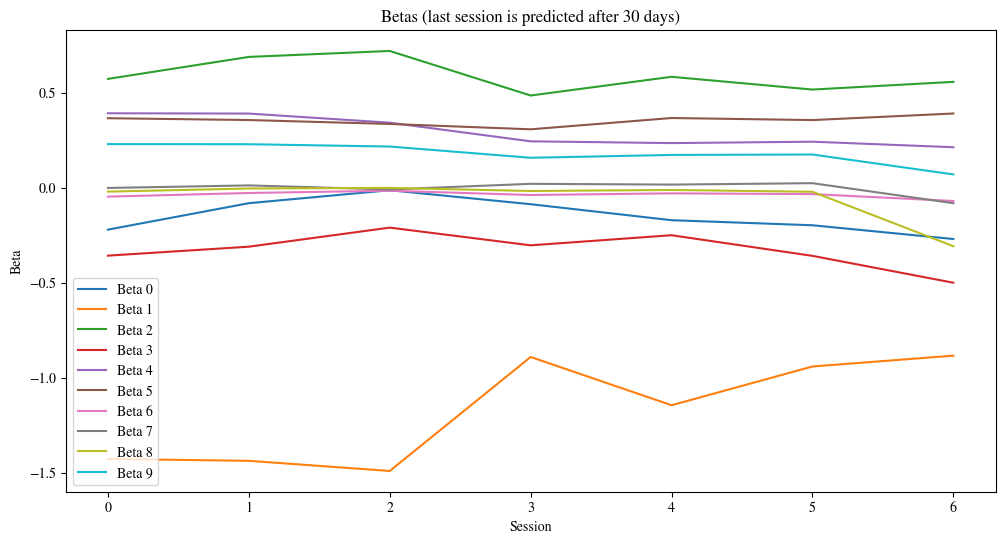
\includegraphics[width=\textwidth]{files/predicted_betas}
    \caption{Change of the shape parameters for a given patient and the neural
        network prediction after 30 days}
\end{figure}